
%----------------------------------------------------------------------------------------%
% START LaTeX preamble

% define document type, font and paper size
\documentclass[11pt,a4paper]{article}

%----------------------------------------------------------------------------------------%
% IMPORT LaTeX packages

\usepackage{inputenc}
\usepackage[ngerman, english]{babel}
\usepackage{csquotes}
\usepackage{amsmath}
\usepackage{amssymb}
\usepackage{amsfonts}
\usepackage{graphicx}
\usepackage{wrapfig}
\usepackage[margin=1.25in]{geometry}
\usepackage{pdfpages}
\usepackage{listings}
\usepackage{setspace}
\usepackage{systeme}
\usepackage{mdframed}
\newcommand{\mathsym}[1]{{}}
\newcommand{\unicode}[1]{{}}




%----------------------------------------------------------------------------------------%
% IMPORT LaTeX packages to manange bibliography

% MLA, APA, or IEEE? - https://www.overleaf.com/learn/latex/Biblatex_citation_styles
\usepackage[style=apa, backend=biber]{biblatex}
\addbibresource{bibliography.bib}

%----------------------------------------------------------------------------------------%
% DEFINE header values

% define the cover page values
\title
{
    Homework 03 - Matrix Inversion
}
\author
{    
    Bruno Gonz{\' a}lez Soria (A01169284)  \\
    Antonio Osamu Katagiri Tanaka (A01212611) \\
    Jos{\' e} Ivan Aviles Castrillo (A01749804) \\
    Jes{\' u}s Alberto Mart{\' i}nez Espinosa (A01750270) \\
    Katya Michelle Aguilar P{\' e}rez (A01750272) \\
    \\
    Instructor: Ph.D Daniel L{\' o}pez Aguayo
}
\date{\today}

%----------------------------------------------------------------------------------------%
% USER-DEFINED commands

% Keywords command
\providecommand{\keywords}[1]
{
    \\
    \\
    \small
    \textbf{\textit{Keywords:}} #1
}

%----------------------------------------------------------------------------------------%

\begin{document}
\setlength\parindent{0pt} % Set noindent for entire file

%----------------------------------------------------------------------------------------%
% CREATE the 1st page (cover page)

\maketitle

%----------------------------------------------------------------------------------------%
% DEFINE the abstract text & keywords

%\begin{abstract}
%    \emph
%    {
%        Lorem ipsum dolor sit amet, consectetur adipiscing elit, sed do eiusmod tempor incididunt ut labore et dolore magna aliqua. Ut enim ad minim veniam, quis nostrud exercitation ullamco laboris nisi ut aliquip ex ea commodo consequat. Duis aute irure dolor in reprehenderit in voluptate velit esse cillum dolore eu fugiat nulla pariatur. Excepteur sint occaecat cupidatat non proident, sunt in culpa qui officia deserunt mollit anim id est laborum.
%    }
%    \keywords{Lorem, ipsum, dolor, sit, amet}
%\end{abstract}
\clearpage

%----------------------------------------------------------------------------------------%
% CREATE a table of contents in a new page

%\tableofcontents
%\clearpage

%----------------------------------------------------------------------------------------%
% CREATE a list of figures and a list of tables in a new page

%\listoffigures
%\listoftables
%\clearpage

%----------------------------------------------------------------------------------------%
% DOCUMENT body starts here

%----------------------------------------------------------------------------------------%
%Append the HW's exercises
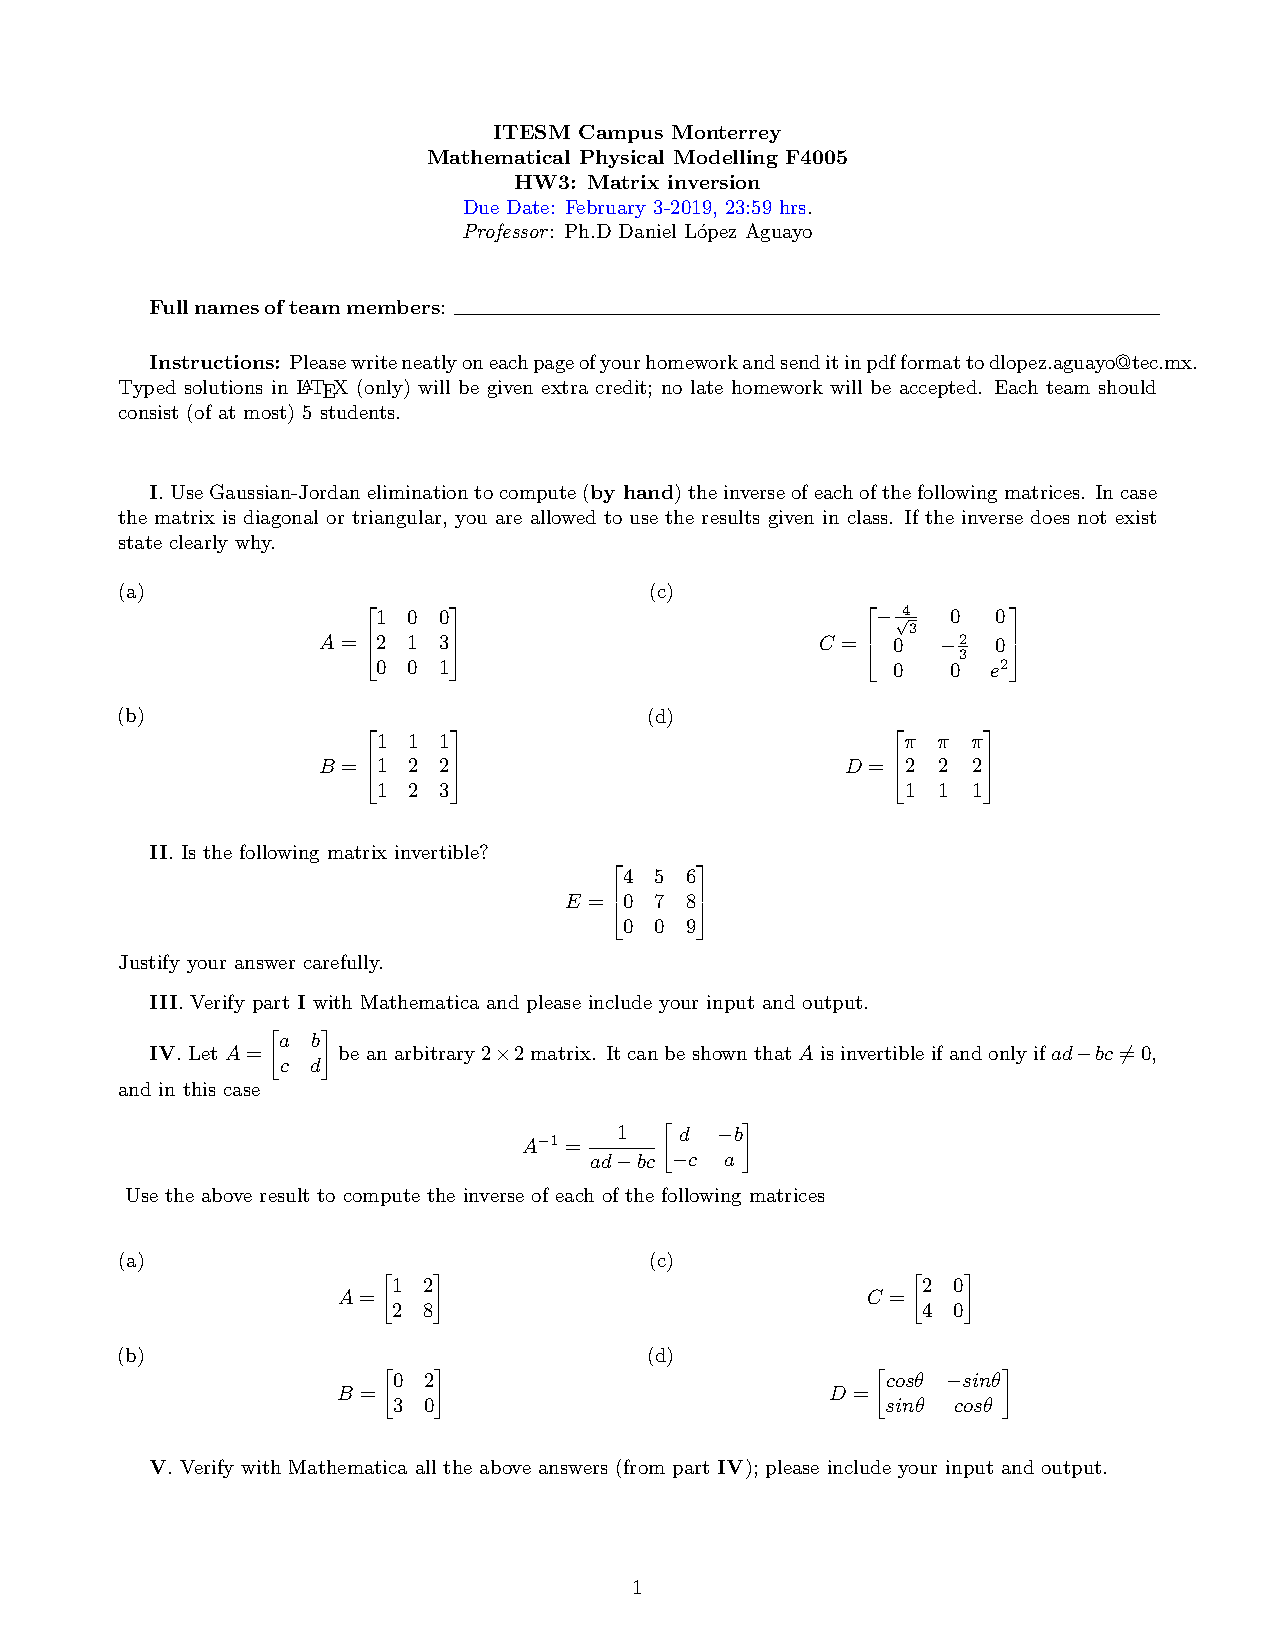
\includepdf[page=-]{HW3}

%----------------------------------------------------------------------------------------%
\section{Answer to Problem I}\label{sec:P01} %Osamu



\clearpage
%----------------------------------------------------------------------------------------%
\section{Answer to Problem II}\label{sec:P02} %Osamu



\clearpage
%----------------------------------------------------------------------------------------%
\section{Answer to Problem III}\label{sec:P03}



\clearpage
%----------------------------------------------------------------------------------------%
\section{Answer to Problem IV}\label{sec:P04}



\clearpage
%----------------------------------------------------------------------------------------%
\section{Answer to Problem V}\label{sec:P05}



\clearpage
%----------------------------------------------------------------------------------------%
\section{Answer to Problem VI}\label{sec:P06}



\clearpage
%----------------------------------------------------------------------------------------%
\section{Answer to Problem VII}\label{sec:P07}



\clearpage
%----------------------------------------------------------------------------------------%
\section{Answer to Problem VIII}\label{sec:P08} %Osamu



\clearpage
%----------------------------------------------------------------------------------------%
\section{Answer to Problem IX}\label{sec:P09}



\clearpage
%----------------------------------------------------------------------------------------%
\section{Answer to Problem X}\label{sec:P10}



\clearpage
%----------------------------------------------------------------------------------------%
% PRINT bibliography/references in a new page

%\clearpage
\printbibliography

%----------------------------------------------------------------------------------------%

\end{document}

%----------------------------------------------------------------------------------------%
